\documentclass[12pt]{article}
\usepackage[utf8]{inputenc}
\usepackage{graphicx}
\usepackage{siunitx}
\usepackage{float}
\usepackage{authblk}
\graphicspath{ {images/} }

\bibliographystyle{plain}

\newenvironment{boxed}
{\begin{center}
		\begin{tabular}{|p{0.9\textwidth}|}
			\hline\\
		}
		{ 
			\\\\\hline
		\end{tabular} 
	\end{center}
}

\begin{document}
\title{Nest detection and habitat mapping of burrow-nesting seabirds using aerial drone based imagery}

\author{Jiménez López, Jesús[1]; García Perez, Agapito[2]}

\affil[1]{Department of Arcane Biology, University of Miskatonic}
\affil[2]{Department of Astrobiology, University of Lebrija}

\maketitle
\begin{abstract}
	
See https://github.com/jesusjl/proyecto\_final

In the last decade, drones (also known as unmanned aerial systems, remotely piloted aircraft systems, RPAS, UAS, UAV) have been the subject of a growing interest in both the civilian and scientific sphere. Drones offer a relatively risk-free and low-cost manner to rapidly and systematically observe natural phenomena at high spatio-temporal resolution. In this study, a drone was used to capture aerial footage to count North Atlantic White-faced Storm-petrel ground nests and describe habitat-specific environmental conditions.

\end{abstract}

{\bf Keywords:} drones, UAV, remote sensing, wildlife monitoring, conservation, island ecology, Pelagodroma marina, burrow nesting seabirds, Selvagem Grande; Macaronesia, Pitingo

\section{Introduction}

The North Atlantic White-faced Storm-petrel (Pelagodroma marina hypoleuca) digs burrow nests in extremely frangible sandy soils, typically forming dense colonies that are often confined to remote and inhabited islands and islets \cite{miguel_pessanha_pais_aquasig_2020}. Conservation and management efforts require regular monitoring of their nests to assess their breeding status and success, as well as possible impacts of anthropogenic pressures \cite{ferreira_bottom-up_2015}. However, fieldwork and censuses are infrequent and with considerable risk of nest trampling. In this context, drone-based aerial imagery surveys can be a non-intrusive, reliable, and effective method of counting nests where close inspection is impractical or constitutes an unacceptable risk of nest disruption and habitat disturbance \cite{ventura_mapping_2018}. 

In this study, a drone was used to collect aerial photographs to assess the feasibility of detecting and counting nests in the imagery and describe habitat-specific environmental conditions. An ortho-photomosaic of the target nesting area was generated, confirming that in stark contrast to sandy soils and surrounding patches of vegetation, burrows were explicitly visible. Hence, burrows were exhaustively counted by visual inspection and compared with semi-automatic detection methods. In addition, object-based image analysis (OBIA) was applied to the ortho-photomosaic to produce a detailed map of vegetation and landforms. Ecological and environmental conditions driving the spatial distribution of the nests were explored to unravel apparent clustering patterns. We discuss the potential and limitations in the use of drones to detect burrowing nests and mapping breeding areas in remote unpopulated islands, and provide guidelines for improved data acquisition to monitor Important Bird and Biodiversity Area (IBA) over time. 

Our study case illustrates that regular scientific ecological information from conspicuous burrow-nesting seabirds can be acquired using very high-resolution aerial images and different processing analytical tools, with minimal disturbance and reduced risks to the nests integrity, contributing therefore to the conservation of North Atlantic White-faced Storm-petrel.

\section{Materials and Methods}

\subsection{Study Site}

Located in the North Atlantic Ocean, the Portuguese Archipelago of Selvagens (\ang{30;8;46.68}N \ang{15;51;51.8}W) are the smaller group of islands in the Macaronesian region, 280 kilometres  south of Madeira, and 165 kilometres north of  the Canary Islands. The archipelago includes two major cluster of islands and islets (Selvagem Grande and Selvagem Pequena) where the White-faced Storm-petrel are know to burrow their nests. In July 2019, we conducted a drone survey in the northernmost colony of the two main breeding areas in Selvagem Grande.  Since flights were performed in the daylight, bird activity was minimum and no disturbance from drone was observed.

\begin{figure}[h]
	\caption{Study site}
	\centering
	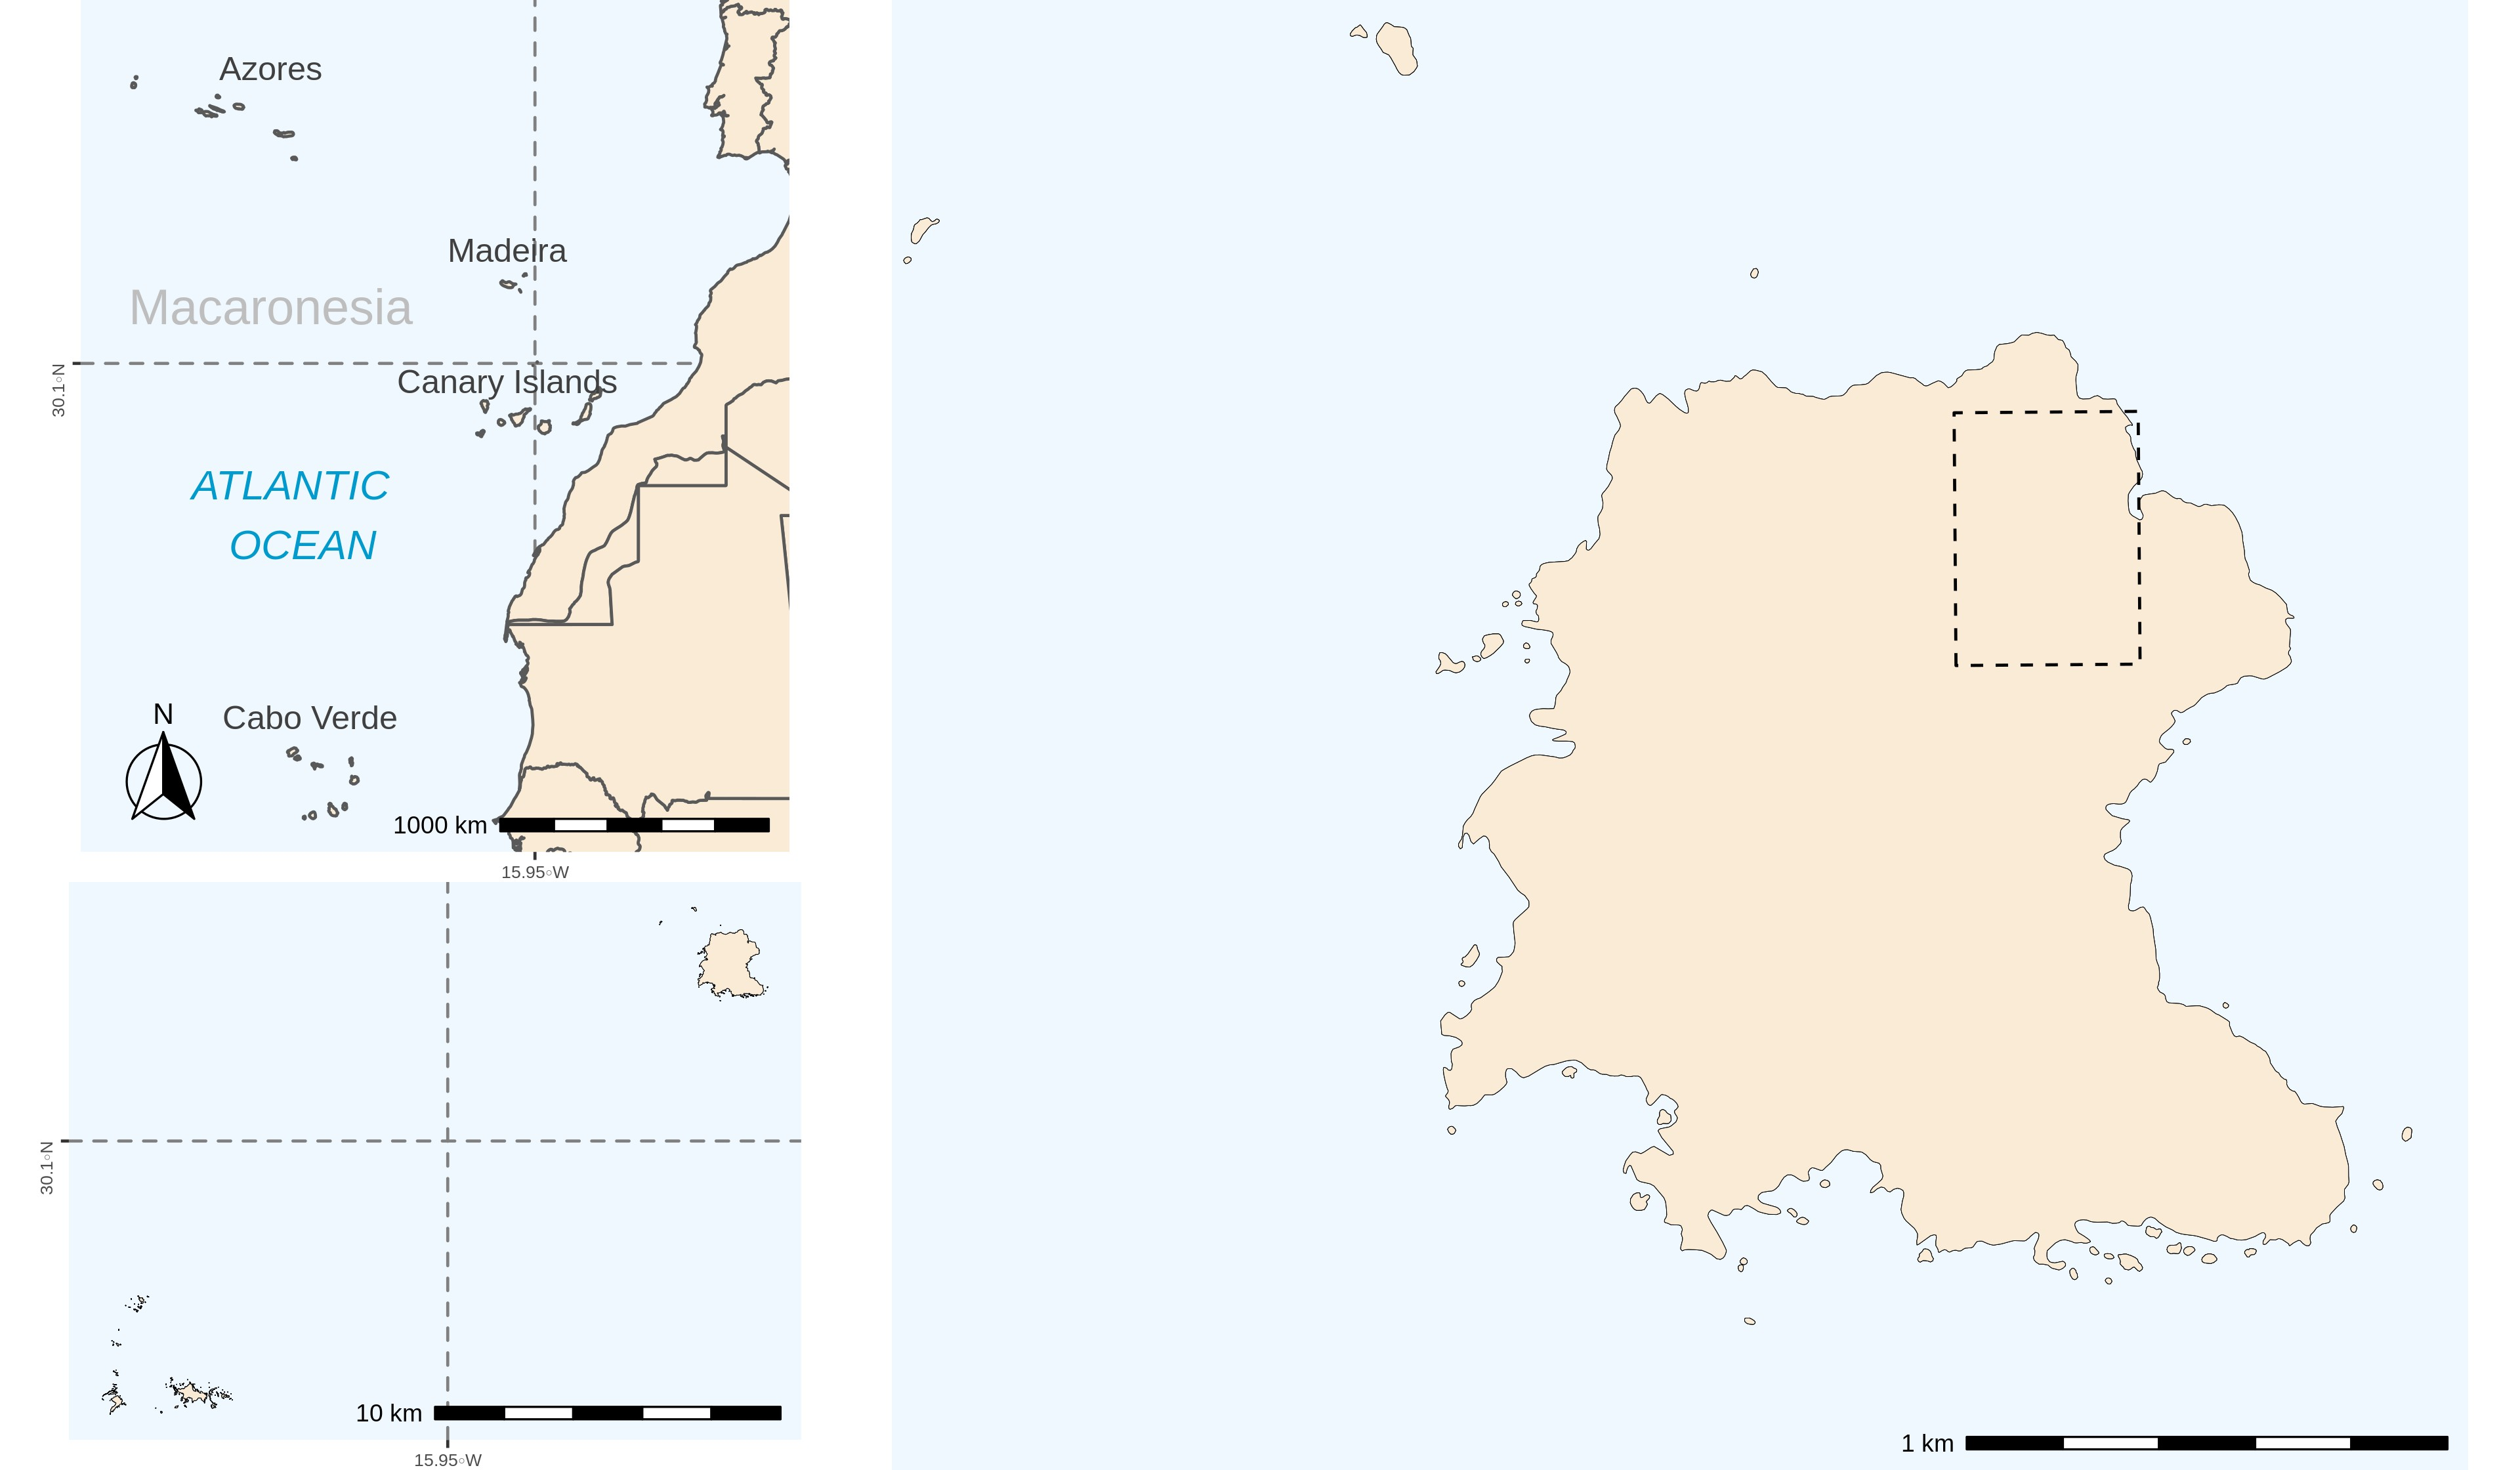
\includegraphics[width=1\textwidth]{map}
\end{figure}


\subsection{Aerial survey and post-processing}

\begin{figure}[h]
	\centering
	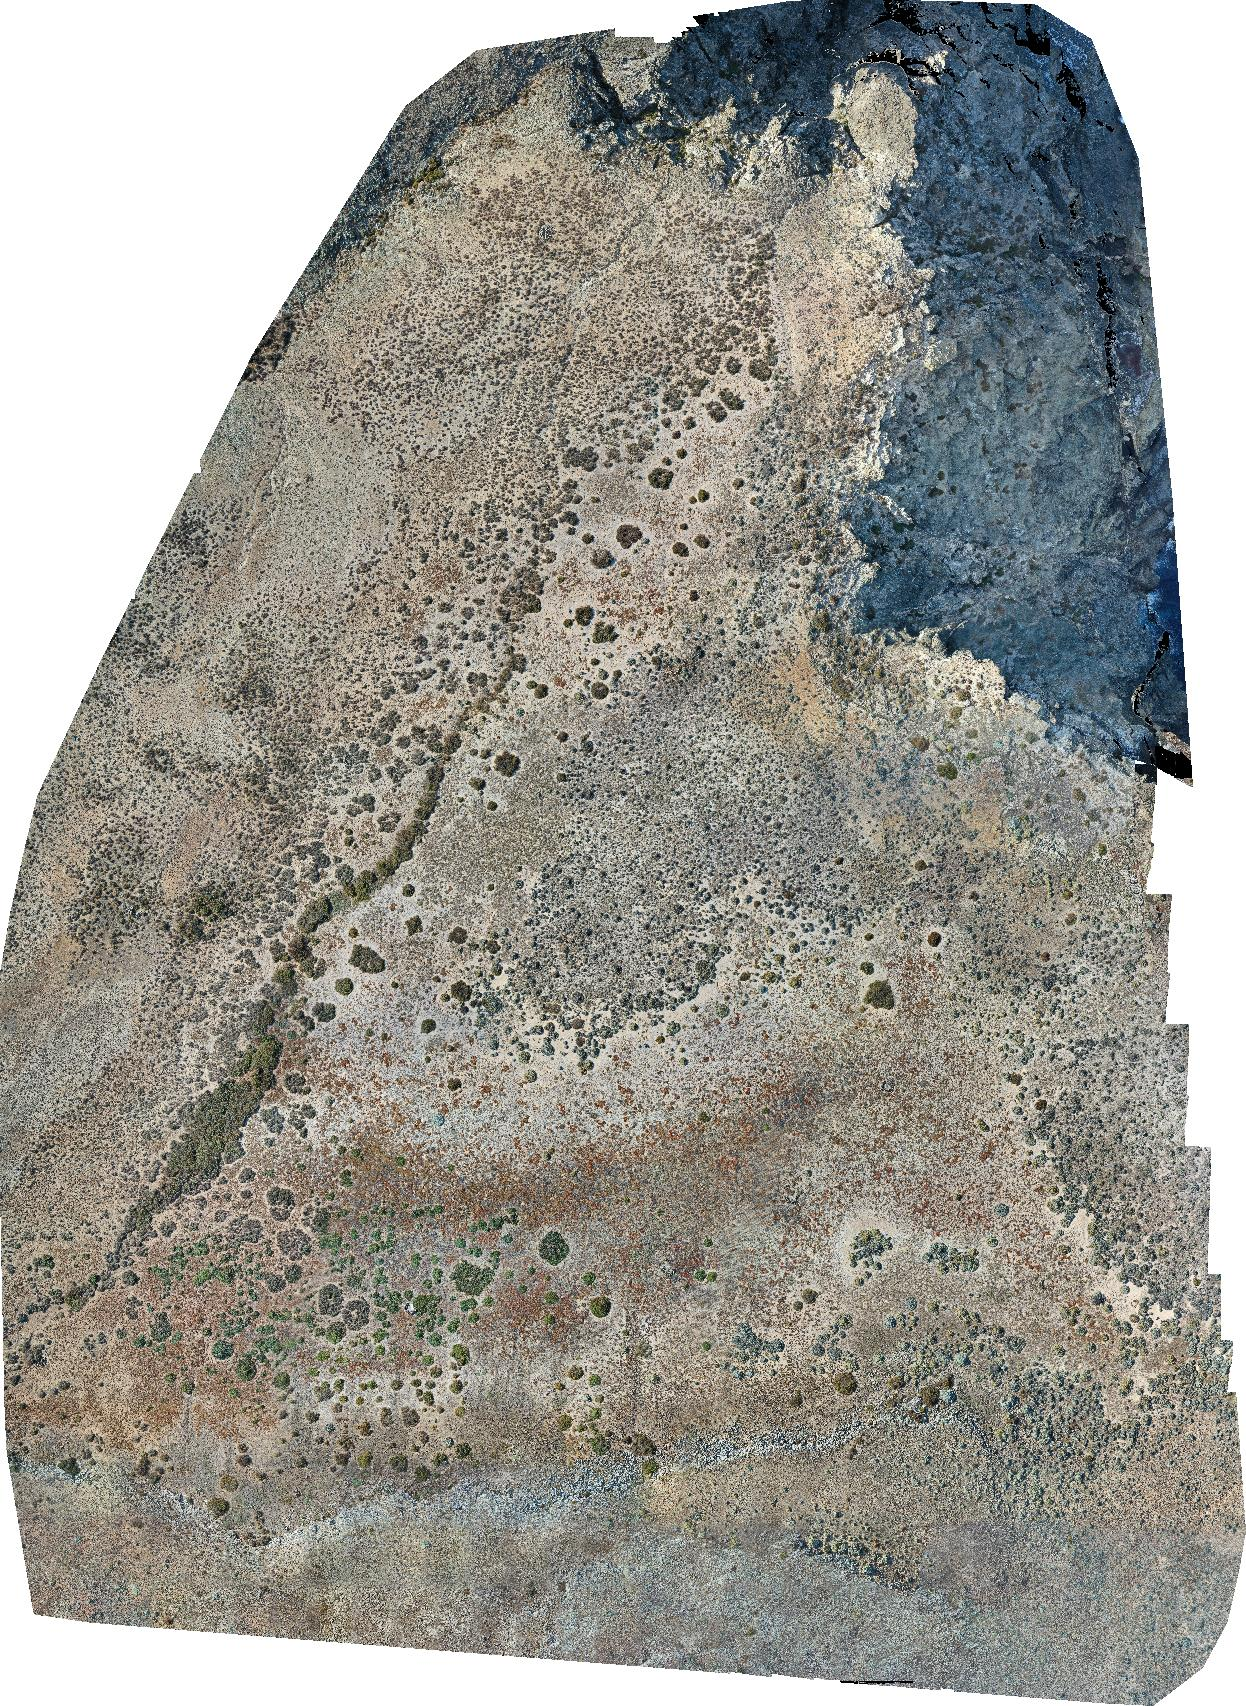
\includegraphics[width=1\textwidth]{mosaic}
	\caption{Mosaic}<
	\label{fig:mosaic}
\end{figure}

\ref{fig:mosaic}

The image acquisition plan consisted in a double grid mission (50 meters altitude) using a consumer-grade drone (DJI Mavic 2 pro) equipped with an RGB sensor. The geotagged images were loaded in Pix4DMapper, a software aimed to generate the 3D models, orthophoto (see figure \ref{fig:mosaic}) and digital terrain model (DTM). Ground control points were taken to eaccurately map the study area ( \ref{tab:table1})) . Additionally, very low altitude flights were carried out for gathering additional imagery and confirm the presence of nests and land-cover classes.

\begin{table}[h!]
	\begin{center}
		\caption{Ground Control Points}
		\label{tab:table1}
		\begin{tabular}{l|c|c|r}
			\textbf{Number} & \textbf{Longitude} & \textbf{Latitude}  & \textbf{Altitude}\\
			\hline
			1 & -15.8608193 & 30.150718 & 88\\
			2 & -15.8623988 & 30.1508263 & 92\\
			3 & -15.8614119 & 30.15204793 & 83\\
			4 & -15.8617023 & 30.1498872 & 98\\
			5 & -15.8598866 & 30.14990833 & 89\\
			6 & -15.8633286 & 30.14997743 & 98\\
			7 & -15.8632504 & 30.14964434 & 98\\
		\end{tabular}
	\end{center}
\end{table}


\subsection{Nest counting}

Burrow nests spots on the orthophoto were systematically digitized as spatial points shapefiles with the assistance of a  vector grid of equal squared cells (QGIS). Following, we compare the manual counted nest dataset with semi-automatic detection using object based image analysis (OBIA) techniques (eCognition Essential). For this purpose, the vector shapefile was split in training and validation sets and respectively used for the image segmentation / classification and accuracy assessment phases.

\begin{figure}[H]
	\caption{Burrow nests are visible}
	\centering
	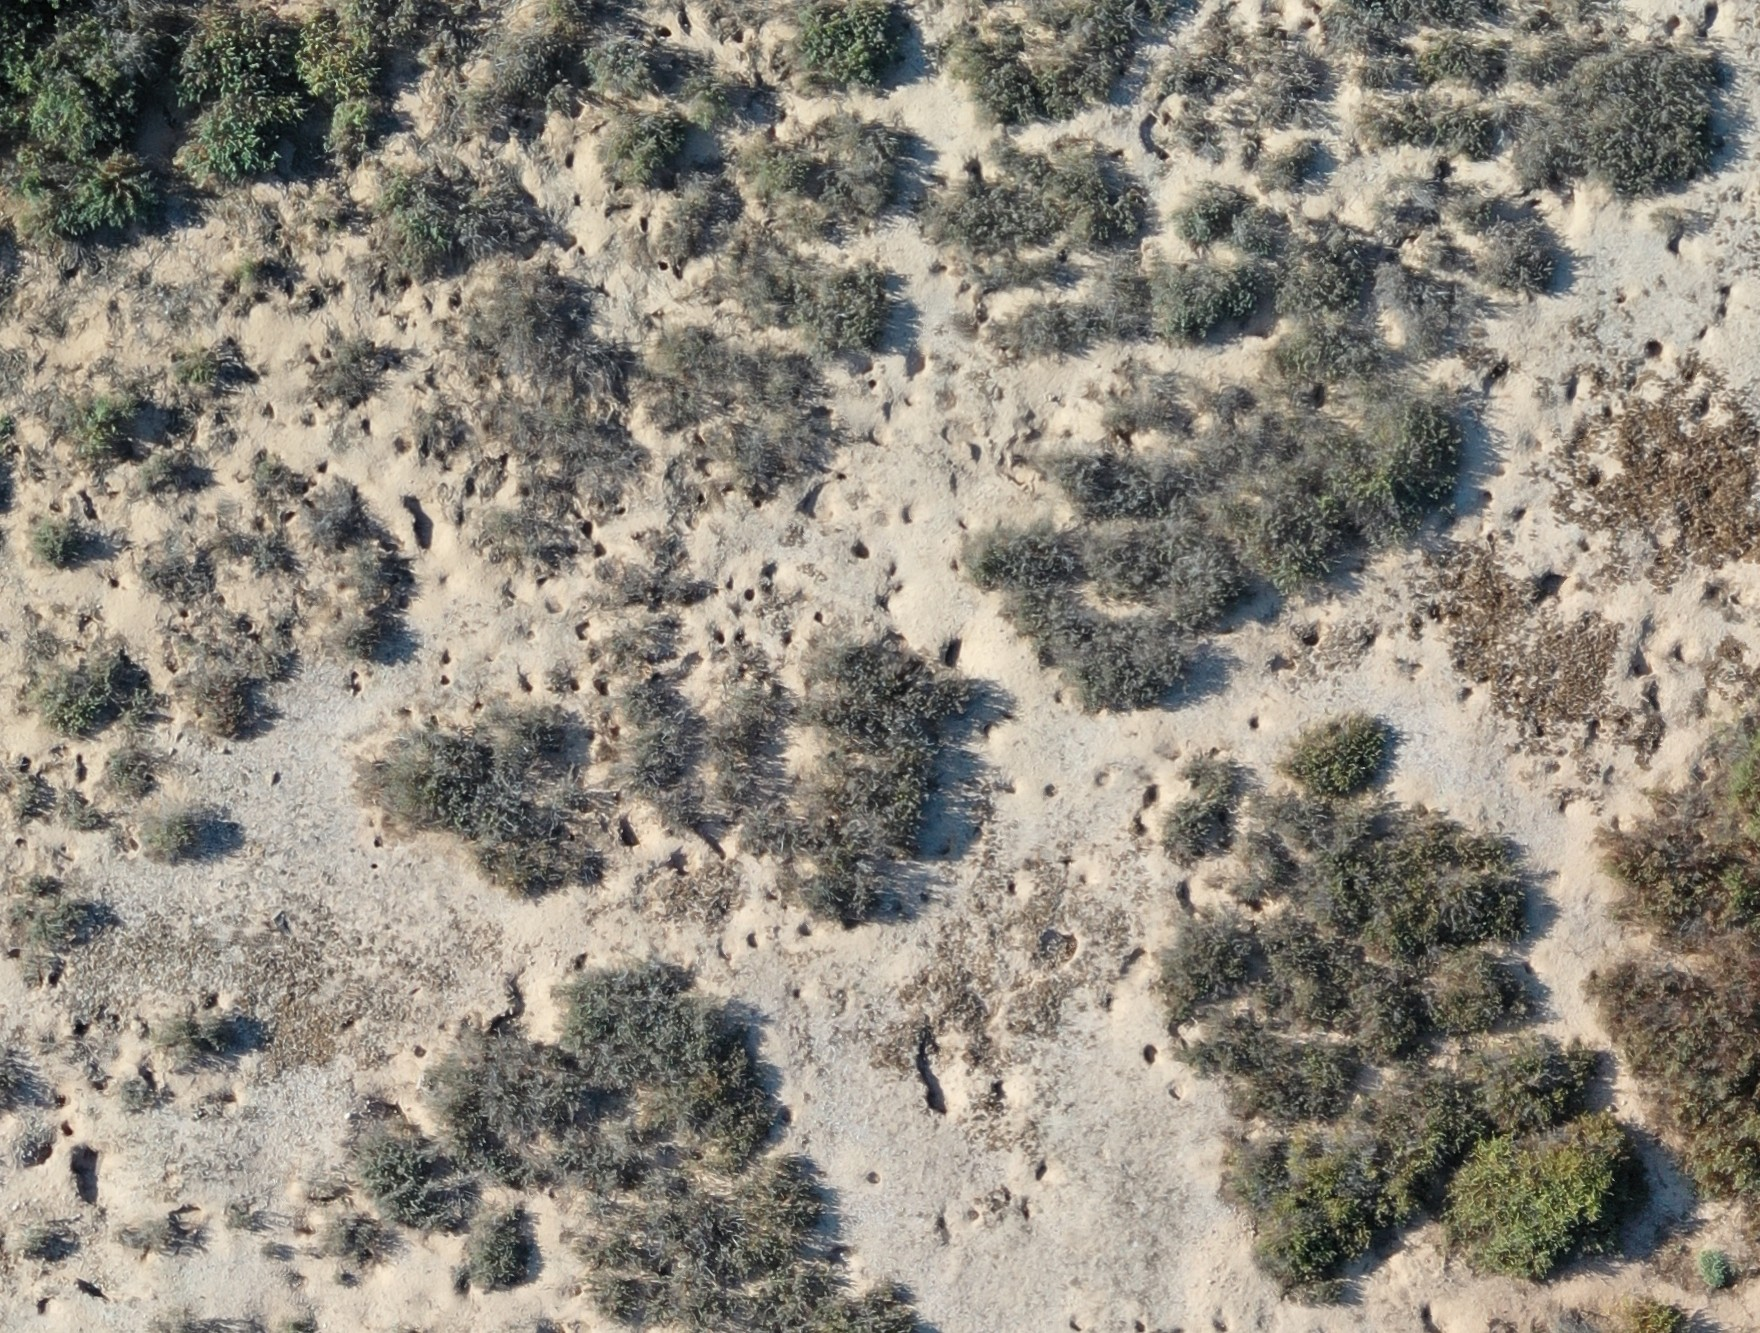
\includegraphics[width=1\textwidth]{clipped_birds_mosaic}
\end{figure}



\subsection{Habitat mapping}

Similar, an habitat map of the study area was produced using OBIA and machine learning techniques. As the very high resolution mosaic permit to clearly differentiate main land cover classes, training data was collected from the same image. 

\subsection{Landscape metrics}

The classified habitat map was used to generate landscape metrics such as area metrics, patch density, size and variability metrics, edge metrics, shape metrics, core area metrics, diversity metrics, and contagion and interspersion metrics. We used \textsf{R} \cite{R_2021} and  \textit{landscapemetrics} package \cite{landscapemetrics_2019}


\begin{boxed}

\textbf{Landscape metrics}

\\

Examples of texture measures supported by \textit{landscapemetrics} package:

\\

Relative Richness: $R=n/nmax*100$, where n=the number of different classes present in the kernel, nmax=maximum number of classes in entire image

Diversity: $H=-\sum(p*ln(p))$, where: $\sum=$the sum over all classes in the entire image, and $p=$proportion of each class in the kernel

Dominance: $D=Hmax-H$, where: $H=$Diversity, $Hmax=$maximum diversity$=ln(n)$ and $n=$number of different classes present in the kernel

Fragmentation: $F=(n-1)/(c-1)$ where n=number of different classes present in the kernel, c=number of cells considered (9, 25 or 49)

NDC=number of different classes in each 3 x 3, 5 x 5, or 7 x 7 neighborhood (ranges from 1-9, 1-25, 1-49)

CVN=number of cells different from the center cell in each 3x3, 5x5, or 7x7 neighborhood (ranges from 0-8, 0-24, 0-48)

BCM=number of different pairs in each 3x3, 5x5, or 7x7 neighborhood


\end{boxed}

\bibliography{bibliography}

\end{document}